\documentclass[12pt]{article}

\usepackage[portuguese]{babel}
\usepackage[utf8]{inputenc}
\usepackage{amsmath}
\usepackage{commath}
\usepackage[alf]{abntex2cite}
\usepackage{indentfirst}
\usepackage{graphicx}
\usepackage{multicol,lipsum}
\usepackage{subfig}
\usepackage{geometry}
\usepackage[alf]{abntex2cite}


\geometry{
	paper = a4paper,
    inner = 3cm,
    outer = 3cm,
    top = 2cm,
    bottom = 2cm
}

\begin{document}
%\maketitle

\onehalfspacing

\begin{titlepage}
	\begin{center}

		\Huge{Universidade Federal de Alagoas}\\
		\large{Instituto de Computação}\\ 
		\large{Laboratório de Computação Científica e Análise Numérica}\\ 
        \vspace{220pt}
        \textbf{\LARGE{Relatório de acompanhamento de pesquisa}}\\
		%\title{{\large{Título}}}
		\vspace{3,5cm}
	\end{center}
	
	\begin{flushleft}
		\begin{tabbing}
			Aluno: Danilo Fernandes Costa\\
			Professor orientador: Alejandro Frery\\
	\end{tabbing}
 \end{flushleft}
	\vspace{1cm}
	
	\begin{center}
		\vspace{\fill}
			 Dezembro\\
		 2018
			\end{center}
\end{titlepage}

\section{Introdução}

Uma forma interessante de representar-se os dados PolSAR é através da matriz de Kennaugh, visto que é composta apenas por valores reais e preserva a informação de retroespalhamento \cite{ClassificationPolSARGeodesic}. Dada uma matriz de coerência $T$ associada a um pixel da imagem, a sua correspondente matriz de Kennaugh é da forma:

\[K =
\begin{bmatrix}

\frac{ T_{11} + T_{22} + T_{33} }{2} & \Re(T_{12}) & \Re(T_{13}) & \Im(T_{23})\\
\Re(T_{12}) & \frac{T_{11} + T_{22} - T_{33}}{2} & \Re(T_{23}) & \Im(T_{13})\\
\Re(T_{13}) & \Re(T_{23}) & \frac{ T_{11} - T_{22} + T_{33} }{2} & -\Im(T_{12})\\
\Im(T_{23}) & \Im(T_{13}) & -\Im(T_{12}) & \frac{ -T_{11} + T_{22} + T_{33} }{2}\\

\end{bmatrix}
.\]

Dadas as matrizes de Kennaugh $K_1$ e $K_2$, é possível medir a distância entre as mesmas, por meio da distância geodésica, da seguinte forma:
\begin{displaymath}
GD(K_1, K_2) = \frac{2}{\pi} \cos^{-1} \left(\frac{Tr(K_1^T K_2)}{\sqrt{Tr(K_1^T K_1)} \sqrt{Tr(K_2^T K_2})} \right).
\end{displaymath}.

Em posse disto, é possível medir a semelhança, a qual é dada por $f(K_1, K_2) = 1 - GD(K_1, K_2)$, entre os dados PolSAR e retroespalhadores prototípicos conhecidos. Dentre estes, temos o triédro, diédro e volume aleatório, cujas matrizes de Kennaugh são, respectivamente:

\[K_a =
\begin{bmatrix}
1 & 0 & 0 & 0\\
0 & 1 & 0 & 0\\
0 & 0 & 1 & 0\\
0 & 0 & 0 & -1\\
\end{bmatrix}
,\]

\[K_b =
\begin{bmatrix}
1 & 0 & 0 & 0\\
0 & 1 & 0 & 0\\
0 & 0 & -1 & 0\\
0 & 0 & 0 & 1\\
\end{bmatrix}
,\]

\[K_{rv} =
\begin{bmatrix}
1 & 0 & 0 & 0\\
0 & 1/2 & 0 & 0\\
0 & 0 & 1/2 & 0\\
0 & 0 & 0 & 0\\
\end{bmatrix}
.\]

No presente relatório são apresentados histogramas das similaridades dos dados de regiões de vegetação e solo exposto em relação aos retroespalhadores prototípicos supracitados. Os dados utilizados foram obtidos em UAVSAR e referem-se a uma região de Sierra del Lacandon National Park, Guatemala.

\section{Histogramas das similaridades}

Para o cálculo das similaridades é necessário que os dados referentes às bandas HHHH, HVHV, VVVV, HHHV, HHVV e HVVV estejam carregados no formato de matrizes na memória. Feito isto, é calculado a intensidade dos dados complexos referentes a esses três últimos obtendo-se seu módulo por meio da função nativa \texttt{Mod} e elevando o resultado ao quadrado. 

Para calcular as similaridades, executou-se o seguinte script:
\begin{verbatim}
mod_kennaugh <- sqrt( hhhh^2 + hvhv^2 + vvvv^2 + 
                      2*int_hhhv + 2*int_hhvv + 2*int_hvvv )

similarity_trihedral <- 1 - (2/pi)*acos( hhhh / mod_kennaugh )
similarity_dihedral  <- 1 - (2/pi)*acos( hvhv / mod_kennaugh )
similarity_rand_vol  <- 1 - (2/pi)*acos( ( 2*hhhh + hvhv + vvvv ) / 
                                         ( sqrt(6)*mod_kennaugh ) ) 
\end{verbatim}

Nas figuras \ref{fig:img1} e \ref{fig:img2} estão indicadas as regiões cujos dados foram utilizados no cálculo das similaridades em relação aos retroespalhores citados.

\begin{figure}[!h]
    \centering
    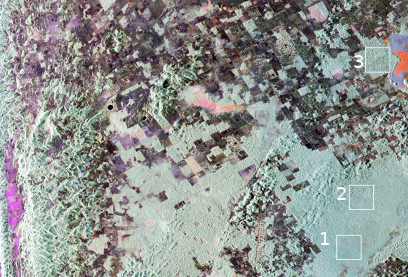
\includegraphics[width = 0.9\linewidth]{../../Images/Report_18_12_17/guatemala2.png}
    \caption{Regiões 1, 2 e 3 selecionadas da Sierra del Lacandon National Park, Guatemala}
    \label{fig:img1}
\end{figure}

\begin{figure}[!h]
    \centering
    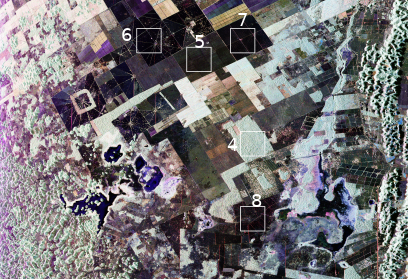
\includegraphics[width = 0.9\linewidth]{../../Images/Report_18_12_17/guatemala1.png}
    \caption{Regiões 4,5,6,7 e 8 selecionadas da Sierra del Lacandon National Park, Guatemala}
    \label{fig:img2}
\end{figure}
\newpage
As figuras \ref{fig:tri_r1}, \ref{fig:tri_r2}, \ref{fig:tri_r3}, \ref{fig:tri_r4} e \ref{fig:tri_r5} apresentam os histogramas das similaridades em relação ao retroespalhador prototípico triédrico dos dados das regiões 1 à 5. Estas correspondem a regiões de vegetação, onde as quatro primeiras correspondem a regiões florestais e a última a uma região de plantação. 
É observável o ajuste desses histogramas a distribuições Normais com parâmetros relativamente próximos. 

\begin{figure}[!h]
    \centering
    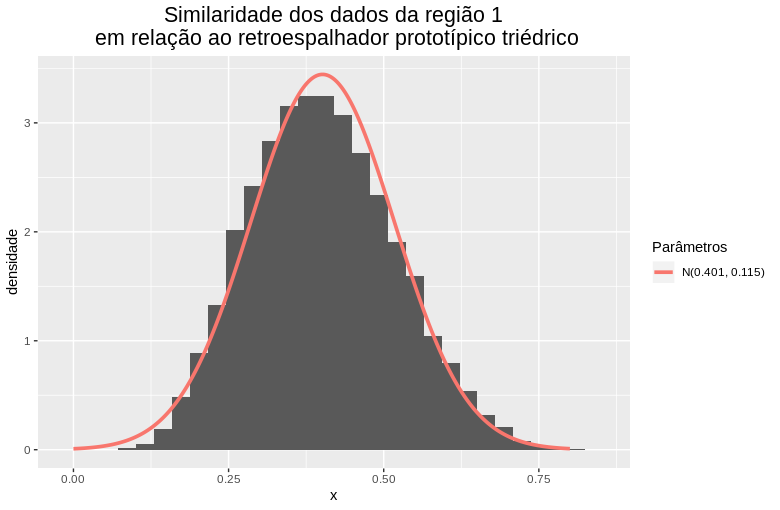
\includegraphics[width = 0.95\linewidth]{../../Images/Report_18_12_17/tri_region1.png}
    \caption{Região 1}
    \label{fig:tri_r1}
\end{figure}

\begin{figure}[!h]
    \centering
    \vspace{0.1\linewidth}
    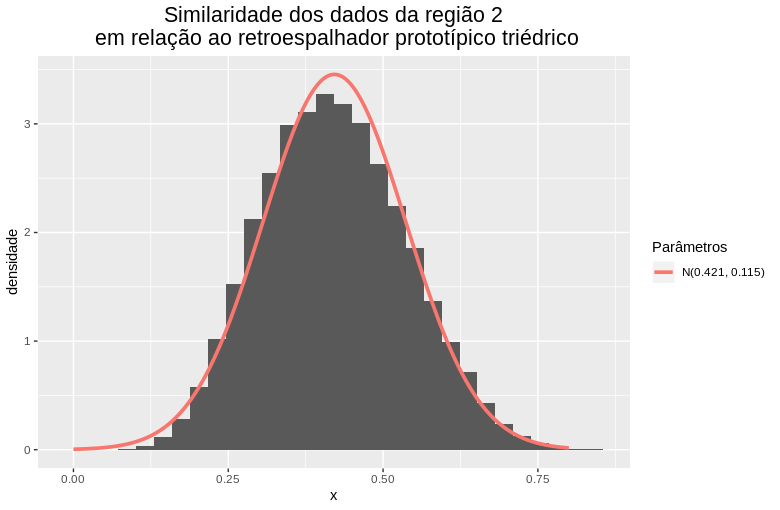
\includegraphics[width = 0.95\linewidth]{../../Images/Report_18_12_17/tri_region2.png}
    \caption{Região 2}
    \label{fig:tri_r2}
\end{figure}

\begin{figure}[!h]
    \centering
    \vspace{0.15\linewidth}
    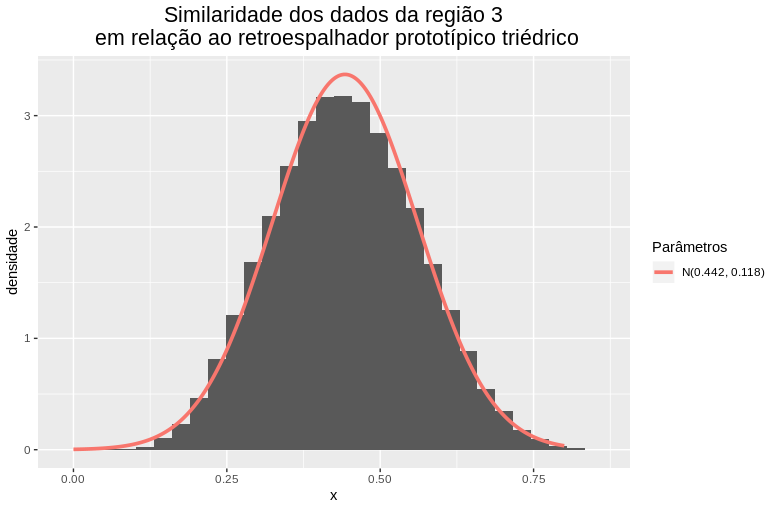
\includegraphics[width = 0.95\linewidth]{../../Images/Report_18_12_17/tri_region3.png}
    \caption{Região 3}
    \label{fig:tri_r3}
\end{figure}

\begin{figure}[!h]
    \centering    
    \vspace{0.1\linewidth}
    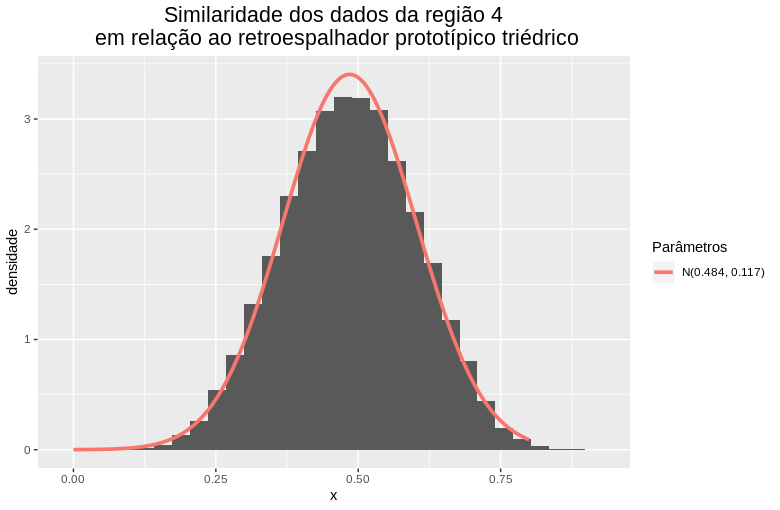
\includegraphics[width = 0.95\linewidth]{../../Images/Report_18_12_17/tri_region4.png}
    \caption{Região 4}
    \label{fig:tri_r4}
\end{figure}

\begin{figure}[!h]
    \centering    
    \vspace{0.1\linewidth}
    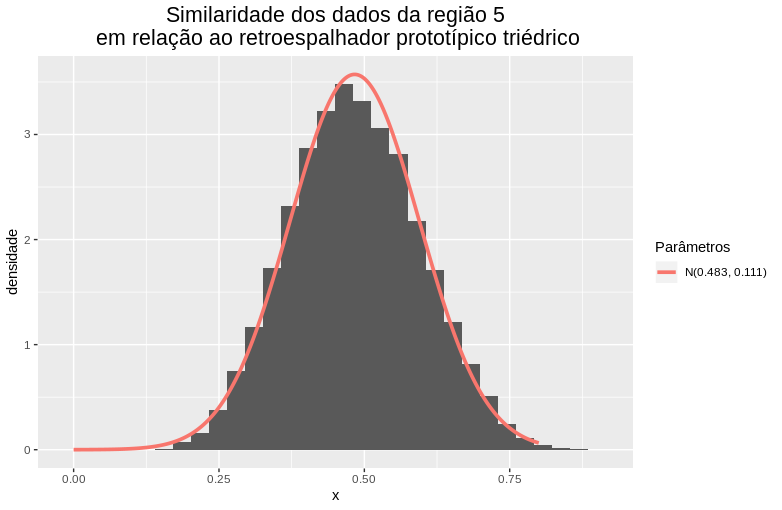
\includegraphics[width = 0.95\linewidth]{../../Images/Report_18_12_17/tri_region5.png}
    \caption{Região 5}
    \label{fig:tri_r5}
\end{figure}

As figuras \ref{fig:di_r1}, \ref{fig:di_r2}, \ref{fig:di_r3}, \ref{fig:di_r4} e \ref{fig:di_r5} apresentam os histogramas das similaridades dos dados das regiões 1 à 5 em relação ao retroespalhador prototípico diédrico. É notório o ajuste dos histogramas a distribuições Gama com parâmetros relativamente próximos, com exceção da região 5. Deve ser observado que esses parâmetros foram estimados utilizando a função \texttt{mle} da bilioteca \texttt{stats4}.

\begin{figure}[!h]
    \centering
    \vspace{0.1\linewidth}
    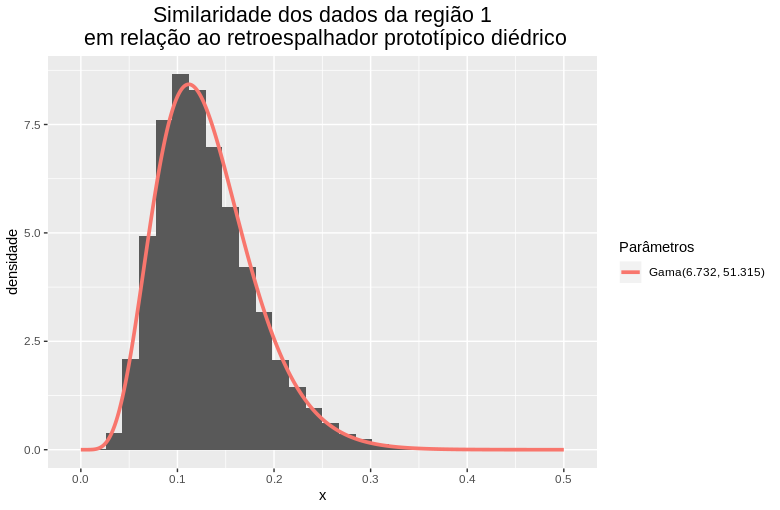
\includegraphics[width = 0.93\linewidth]{../../Images/Report_18_12_17/di_region1.png}
    \caption{Região 1}
    \label{fig:di_r1}
\end{figure}

\begin{figure}[!h]
    \centering
    \vspace{0.05\linewidth}
    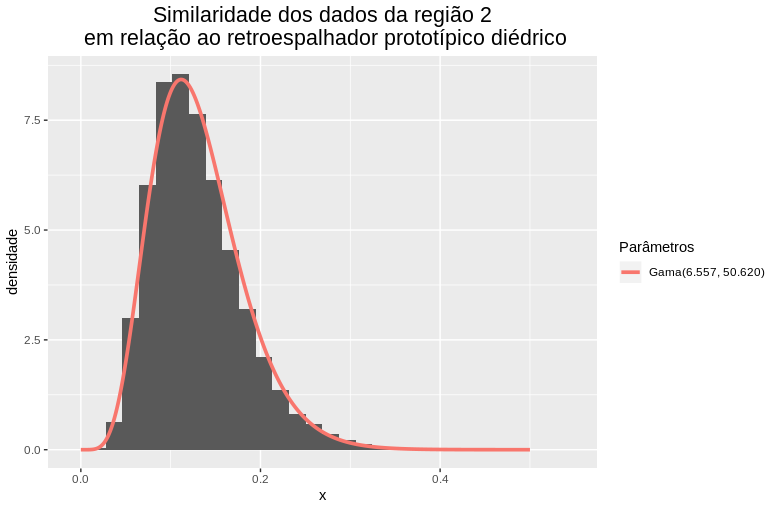
\includegraphics[width = 0.93\linewidth]{../../Images/Report_18_12_17/di_region2.png}
    \caption{Região 2}
    \label{fig:di_r2}
\end{figure}

\begin{figure}[!h]
    \centering
    \vspace{0.1\linewidth}
    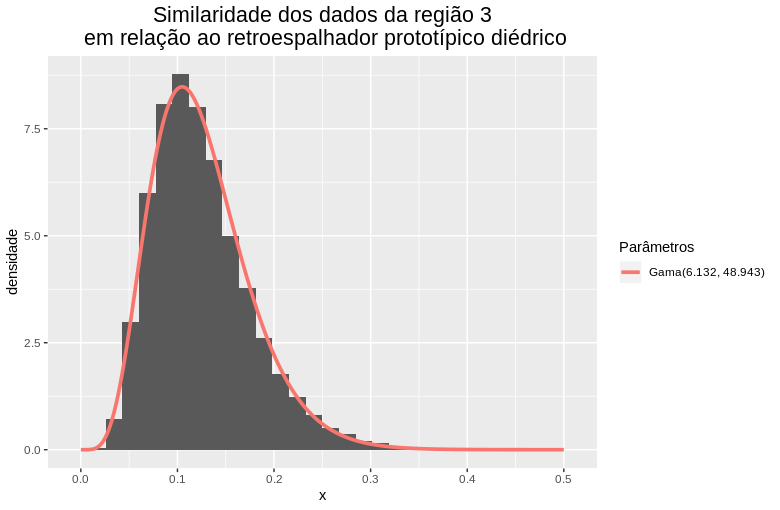
\includegraphics[width = 0.95\linewidth]{../../Images/Report_18_12_17/di_region3.png}
    \caption{Região 3}
    \label{fig:di_r3}
\end{figure}

\begin{figure}[!h]
    \centering
    \vspace{0.15\linewidth}
    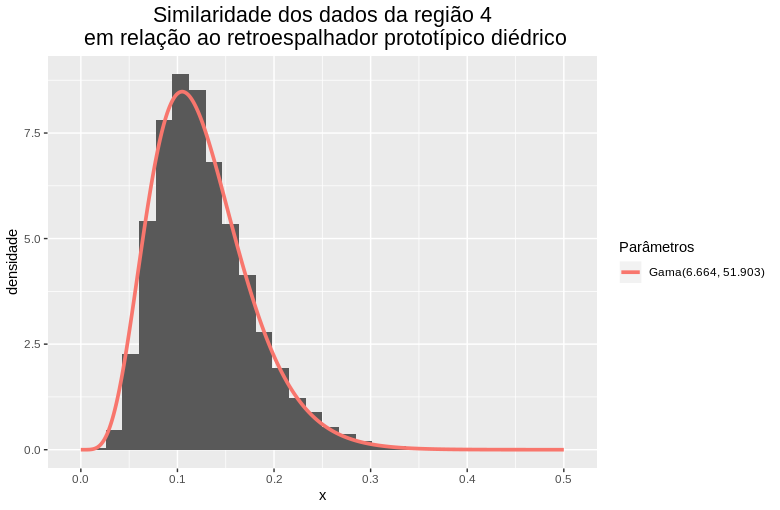
\includegraphics[width = 0.95\linewidth]{../../Images/Report_18_12_17/di_region4.png}
    \caption{Região 4}
    \label{fig:di_r4}
\end{figure}

\begin{figure}[!h]
    \centering
    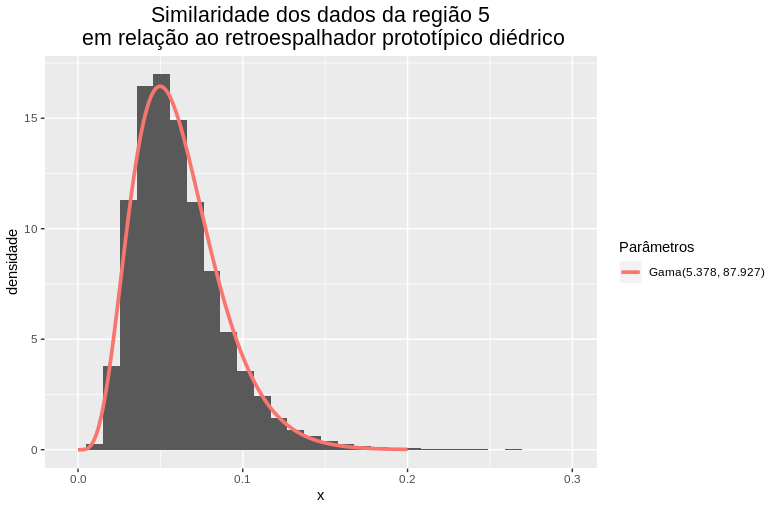
\includegraphics[width = 0.95\linewidth]{../../Images/Report_18_12_17/di_region5.png}
    \caption{Região 5}
    \label{fig:di_r5}
\end{figure}

As figuras \ref{fig:rv_r1}, \ref{fig:rv_r2}, \ref{fig:rv_r3}, \ref{fig:rv_r4} e \ref{fig:rv_r5} apresentam os histogramas das similaridades dos dados das regiões 1 à 5 em relação ao retroespalhador prototípico volume aleatório. Novamente, é possível observar o ajuste dos histogramas a distribuições Normais com parâmetros próximos.

\begin{figure}[!h]
    \centering
    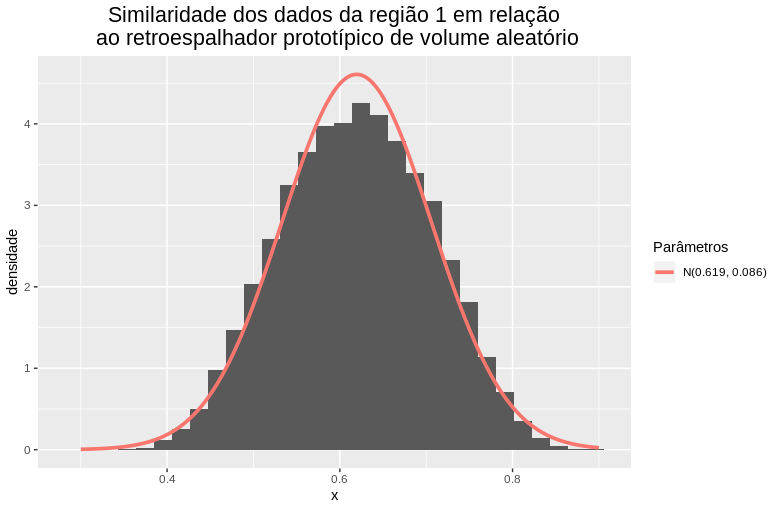
\includegraphics[width = 0.95\linewidth]{../../Images/Report_18_12_17/rv_region1.png}
    \caption{Região 1}
    \label{fig:rv_r1}
\end{figure}

\begin{figure}[!h]
    \centering
    \vspace{0.1\linewidth}
    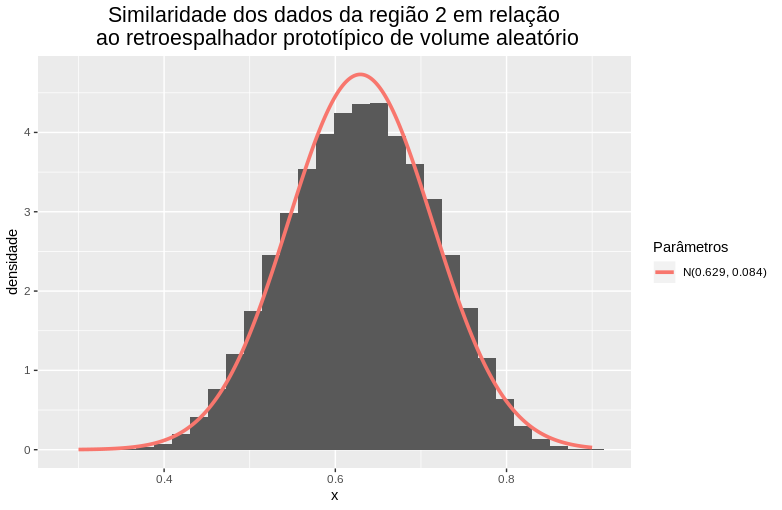
\includegraphics[width = 0.95\linewidth]{../../Images/Report_18_12_17/rv_region2.png}
    \caption{Região 2}
    \label{fig:rv_r2}
\end{figure}

\begin{figure}[!h]
    \centering
    \vspace{0.15\linewidth}
    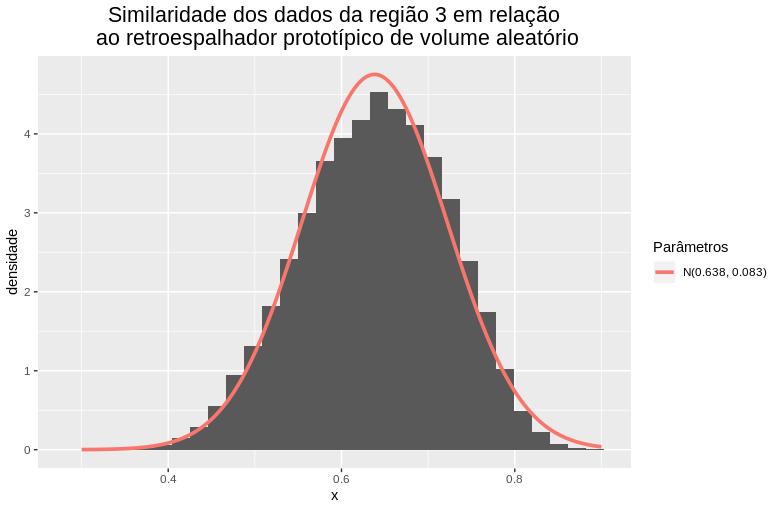
\includegraphics[width = 0.95\linewidth]{../../Images/Report_18_12_17/rv_region3.png}
    \caption{Região 3}
    \label{fig:rv_r3}
\end{figure}

\begin{figure}[!h]
    \centering    
    \vspace{0.1\linewidth}
    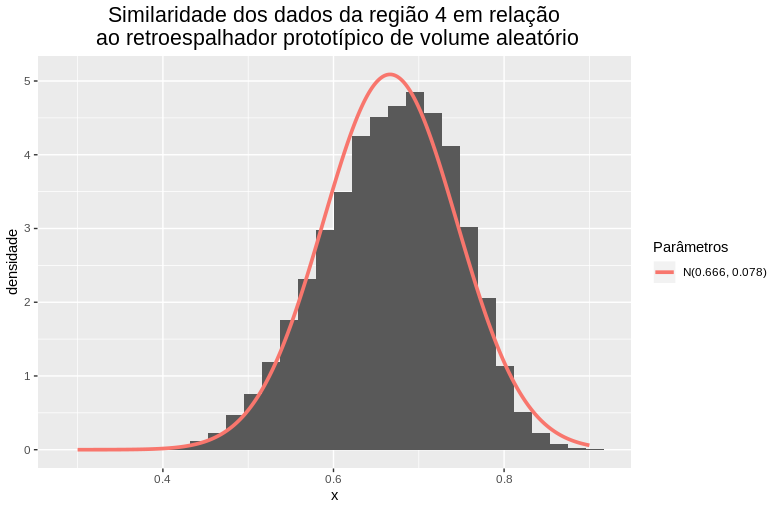
\includegraphics[width = 0.95\linewidth]{../../Images/Report_18_12_17/rv_region4.png}
    \caption{Região 4}
    \label{fig:rv_r4}
\end{figure}

\begin{figure}[!h]
    \centering    
    \vspace{0.1\linewidth}
    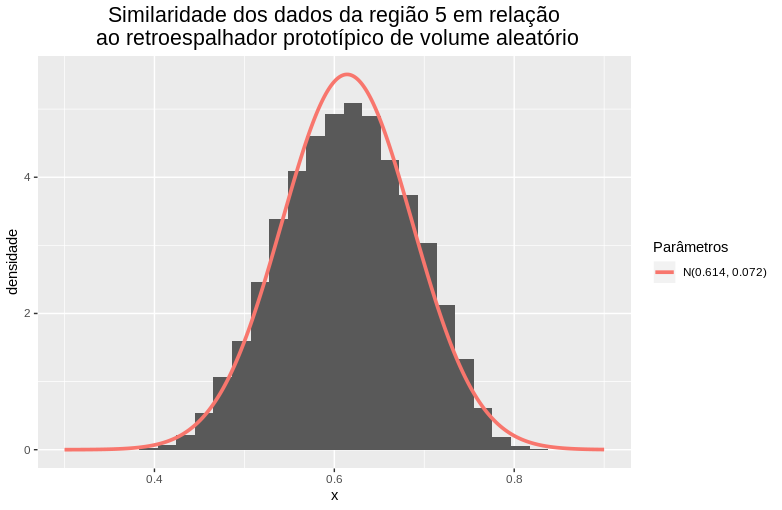
\includegraphics[width = 0.95\linewidth]{../../Images/Report_18_12_17/rv_region5.png}
    \caption{Região 5}
    \label{fig:rv_r5}
\end{figure}

\newpage

As figuras \ref{fig:tri_r6}, \ref{fig:tri_r7} e \ref{fig:tri_r8} apresentam os histogramas das similaridades dos dados das regiões 6 à 8, as quais são regiões de solo exposto, em relação ao retroespalhador prototípico triédrico. Observemos que há uma considerável variabilidade nos parâmetros e que não houve ajuste à distribuição Gama no histograma da figura \ref{fig:tri_r6}. 

\begin{figure}[!h]
    \centering
    \vspace{0.05\linewidth}
    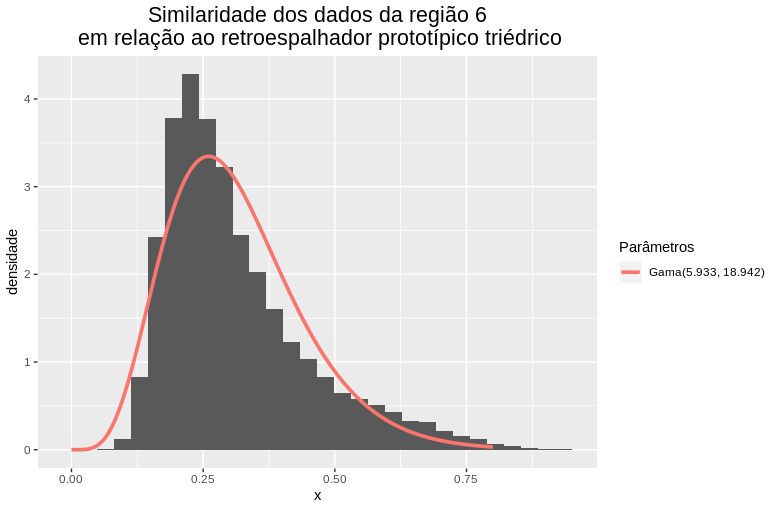
\includegraphics[width = 0.95\linewidth]{../../Images/Report_18_12_17/tri_region6.png}
    \caption{Região 6}
    \label{fig:tri_r6}
\end{figure}

\begin{figure}[!h]
    \centering
    \vspace{0.1\linewidth}
    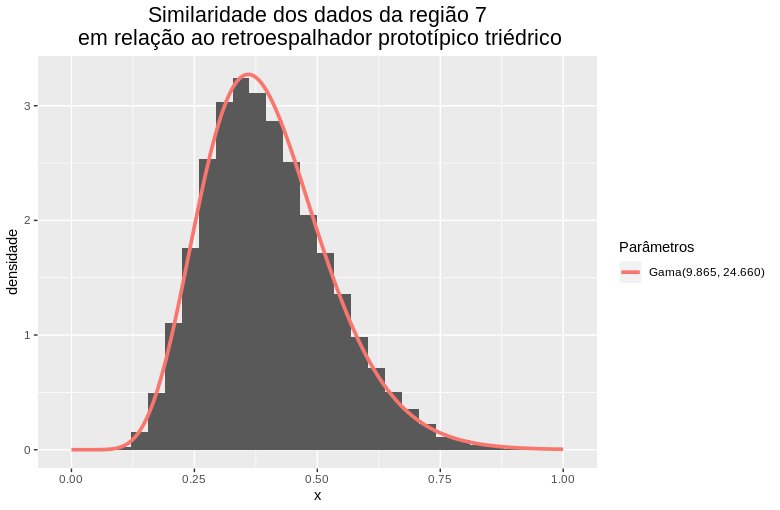
\includegraphics[width = 0.95\linewidth]{../../Images/Report_18_12_17/tri_region7.png}
    \caption{Região 7}
    \label{fig:tri_r7}
\end{figure}

\begin{figure}[!h]
    \centering    
    \vspace{0.1\linewidth}
    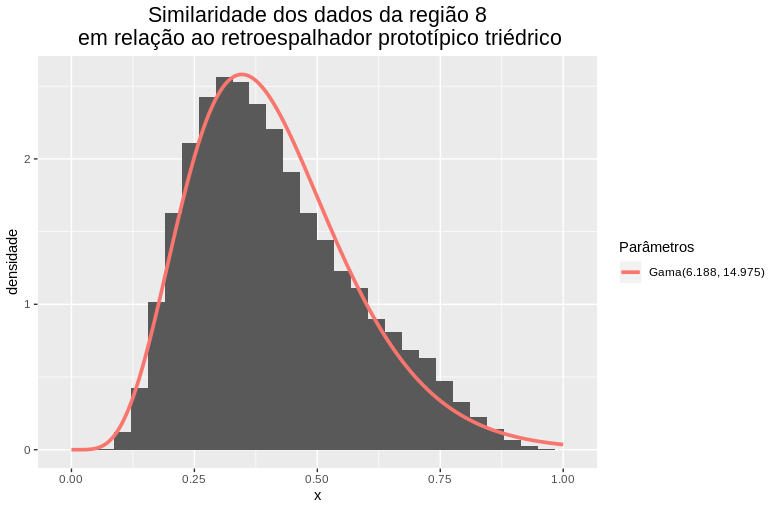
\includegraphics[width = 0.95\linewidth]{../../Images/Report_18_12_17/tri_region8.png}
    \caption{Região 8}
    \label{fig:tri_r8}
\end{figure}

As figuras \ref{fig:di_r6}, \ref{fig:di_r7} e \ref{fig:di_r8} apresentam os histogramas das similaridades dos dados das regiões 6 à 8 em relação ao retroespalhador prototípico diédrico. Embora haja o ajuste a distribuição Gama, também há considerável variabilidade nos parâmetros.

\begin{figure}[!h]
    \centering
    \vspace{0.05\linewidth}
    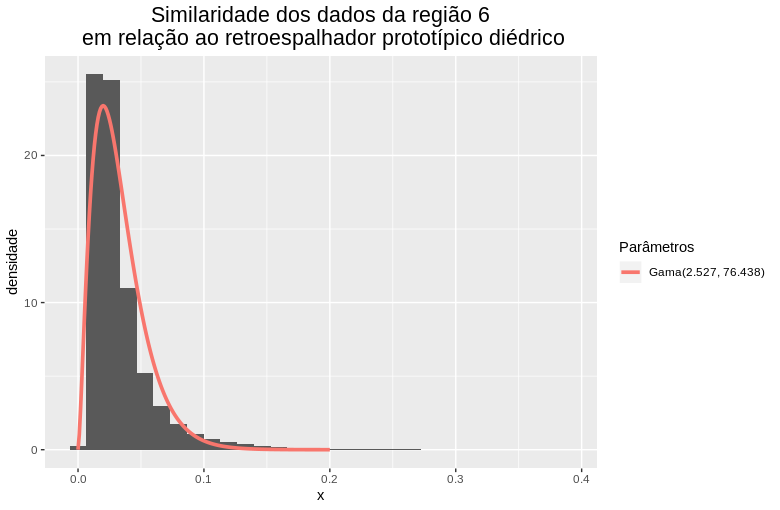
\includegraphics[width = 0.95\linewidth]{../../Images/Report_18_12_17/di_region6.png}
    \caption{Região 6}
    \label{fig:di_r6}
\end{figure}

\begin{figure}[!h]
    \centering
    \vspace{0.1\linewidth}
    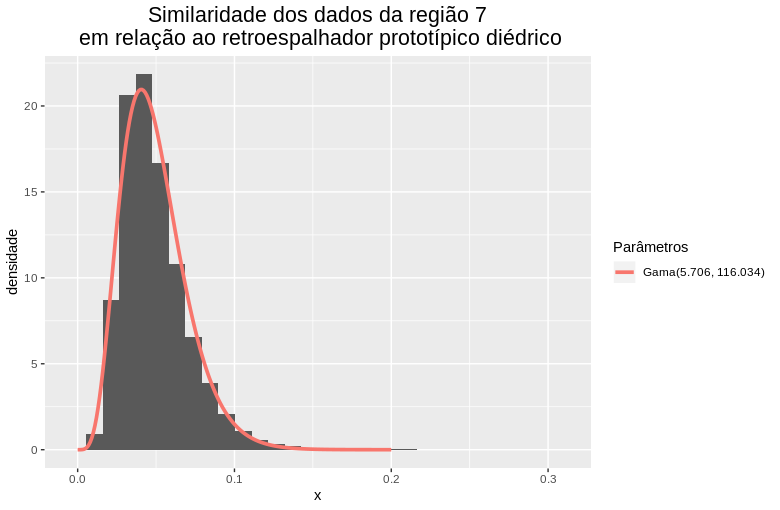
\includegraphics[width = 0.95\linewidth]{../../Images/Report_18_12_17/di_region7.png}
    \caption{Região 7}
    \label{fig:di_r7}
\end{figure}

\begin{figure}[!h]
    \centering    
    \vspace{0.1\linewidth}
    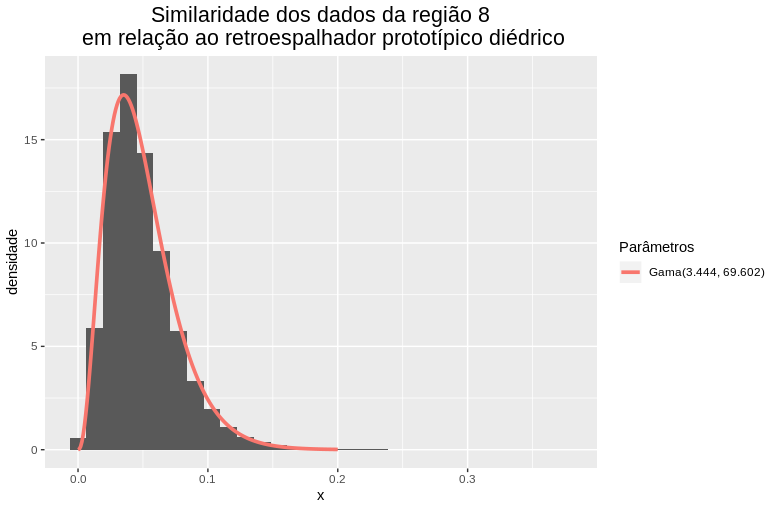
\includegraphics[width = 0.95\linewidth]{../../Images/Report_18_12_17/di_region8.png}
    \caption{Região 8}
    \label{fig:di_r8}
\end{figure}

As figuras \ref{fig:rv_r6}, \ref{fig:rv_r7} e \ref{fig:rv_r8} apresentam os histogramas das similaridades dos dados das regiões 6 à 8 em relação ao retroespalhador prototípico de volume aleatório. Observemos que não houve ajuste dos histogramas à distribuição Gama.

\begin{figure}[!h]
    \centering
    \vspace{0.1\linewidth}
    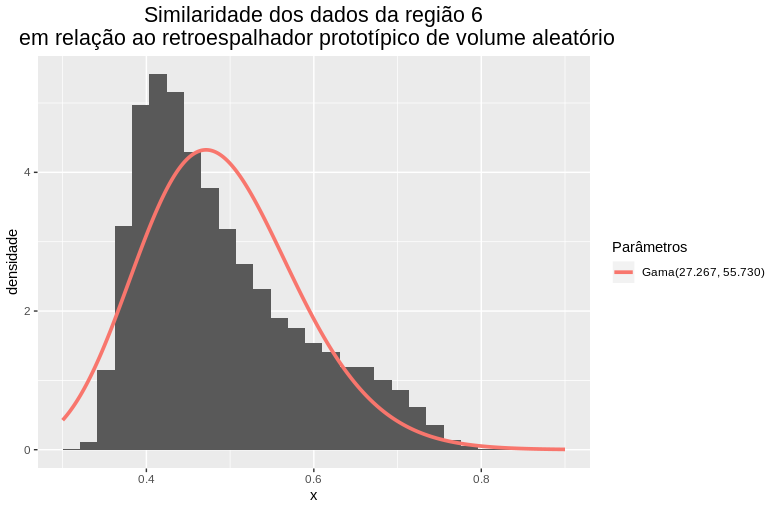
\includegraphics[width = 0.95\linewidth]{../../Images/Report_18_12_17/rv_region6.png}
    \caption{Região 6}
    \label{fig:rv_r6}
\end{figure}

\begin{figure}[!h]
    \centering
    \vspace{0.05\linewidth}
    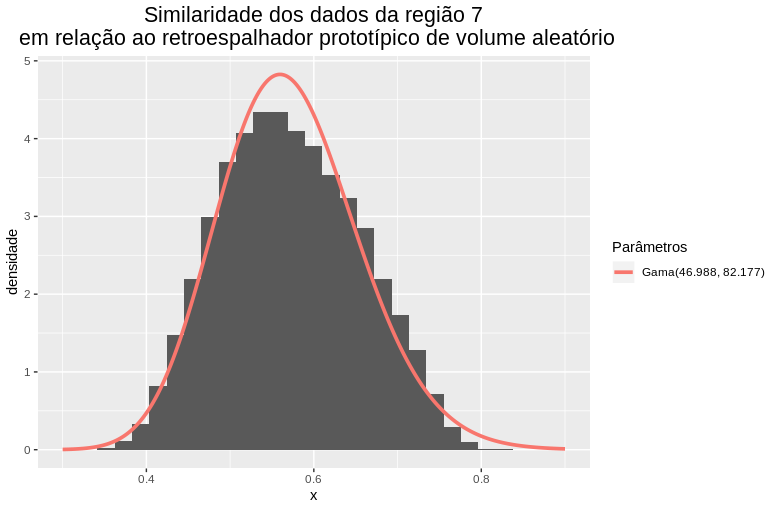
\includegraphics[width = 0.95\linewidth]{../../Images/Report_18_12_17/rv_region7.png}
    \caption{Região 7}
    \label{fig:rv_r7}
\end{figure}

\begin{figure}[!h]
    \centering    
    \vspace{0.1\linewidth}
    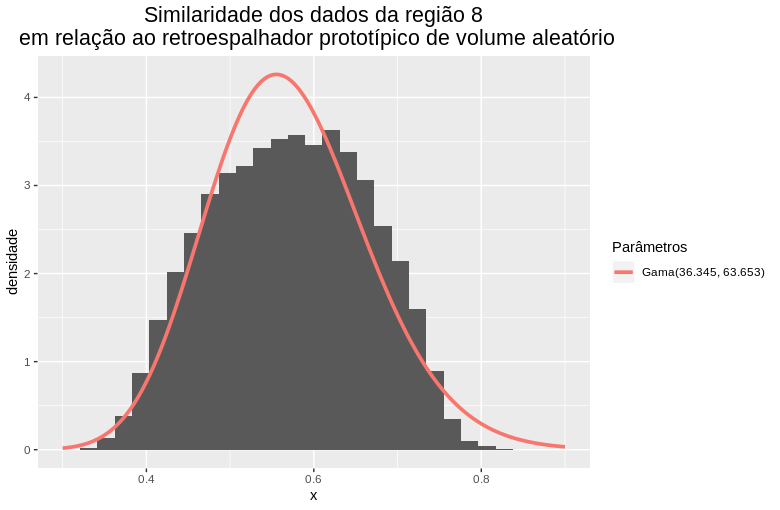
\includegraphics[width = 0.95\linewidth]{../../Images/Report_18_12_17/rv_region8.png}
    \caption{Região 8}
    \label{fig:rv_r8}
\end{figure}

\bibliographystyle{abntex2-alf}
\bibliography{../../Bibliography/ref_18_12_17}

\end{document}
